\documentclass[aspectratio=169,10pt]{beamer}
\usetheme[progressbar=frametitle,numbering=fraction]{metropolis}
\usepackage{booktabs}
\usepackage{tikz}
\usetikzlibrary{arrows.meta,positioning,fit,backgrounds}
\usepackage{pgfplots}
\pgfplotsset{compat=1.17}
\definecolor{accent}{RGB}{31,90,166}
\setbeamercolor{alerted text}{fg=accent}
\setbeamerfont{footnote}{size=\tiny}

\title{Trust but Verify}
\subtitle{Fine-Tuning a Small Vision-Language Model to Weigh Retrieved News Evidence for Image Contextualization}
\author{Bhoomi Kushwaha (MML2025006)\\Aditi Satpathy (MRM2025005)\\Tanuja Churendra (MHC2025008)}
\institute{Department of Information Technology, IIIT Allahabad, Prayagraj}
\date{November 2026}

\begin{document}

% ---------------------------------------------------------------- 1
\maketitle

% ---------------------------------------------------------------- 2
\begin{frame}{Introduction}
\begin{columns}[T]
\column{0.58\textwidth}
\textbf{Task: image contextualization}
\begin{itemize}
\item Given a news photo, predict \alert{where} and \alert{when} it was taken
\item Out-of-context photos (a real image, the wrong place or date) are a common form of misinformation
\item Reverse image search often returns nothing, so we need methods that work without it
\end{itemize}
\vspace{0.6em}
\textbf{Our approach}
\begin{itemize}
\item Retrieve related news articles for the photo
\item Fine-tune a 3B vision-language model to \alert{check} those articles against the photo before answering
\end{itemize}
\column{0.38\textwidth}
\begin{block}{Example output}
\small
\textbf{Input:} news photo, no caption\\[0.3em]
\textbf{Output:}\\
\texttt{Location: Port-au-Prince, Haiti}\\
\texttt{Date: 2010-01-19}\\[0.3em]
plus the 3 supporting articles
\end{block}
\end{columns}
\end{frame}

% ---------------------------------------------------------------- 3
\begin{frame}{Related Work / Base Papers}
\begin{columns}[T]
\column{0.49\textwidth}
\begin{block}{NewsRECON (Tonglet et al., 2026) --- base paper}
\small
\begin{itemize}
\item Links an image to $\sim$90k NYT + Guardian articles
\item CLIP bi-encoder $\rightarrow$ location and event cross-encoders
\item Top-3 articles passed to a \alert{frozen} MLLM (Qwen2.5-VL-7B), prompted zero-shot
\item Evaluated on TARA and 5Pils-OOC with the GREAT metric
\end{itemize}
\end{block}
\column{0.49\textwidth}
\begin{block}{LiveVQA (Fu et al., 2025) --- training recipe}
\small
\begin{itemize}
\item Updates MLLMs with new visual knowledge from news
\item LoRA fine-tuning on three formats: \textbf{QA}, \textbf{MCQA}, \textbf{QAR} (with reasoning)
\item Uses Qwen2.5-VL-3B
\end{itemize}
\end{block}
\end{columns}
\vspace{0.5em}
\small
\textbf{Other related work:} TARA dataset (Fu et al., 2022) $\cdot$ CLIP (Radford et al., 2021) $\cdot$ LoRA (Hu et al., 2022) $\cdot$ knowledge conflicts in RAG (Longpre et al., 2021; Xie et al., 2024) $\cdot$ training with distractor documents, RAFT (Zhang et al., 2024)
\end{frame}

% ---------------------------------------------------------------- 4
\begin{frame}{Research Problem and Motivation}
\begin{columns}[T]
\column{0.55\textwidth}
\textbf{The gap in NewsRECON: ``blind trust''}
\begin{itemize}
\item The MLLM is never trained to judge evidence
\item In \alert{6 of 50} inspected cases, a correct answer from the photo was \alert{overwritten} by a wrong article
\item Bigger models (32B, 72B) did not reliably help
\item Exact date accuracy is only 3--5\%
\end{itemize}
\vspace{0.5em}
\textbf{Research question}\\
Can LiveVQA-style fine-tuning teach a \alert{small} MLLM to use good articles and reject bad ones?
\column{0.42\textwidth}
\begin{alertblock}{Motivation}
\small
\begin{itemize}
\item Retrieval is noisy: only $\sim$54\% of top-3 articles are about the right place, and $\sim$4\% about the right event
\item Fact-checkers need answers that do not copy noisy evidence
\item Limited compute: one 24\,GB GPU, one day
\end{itemize}
\end{alertblock}
\end{columns}
\end{frame}

% ---------------------------------------------------------------- 5
\begin{frame}{Proposed Methodology (1/2): Pipeline}
\centering
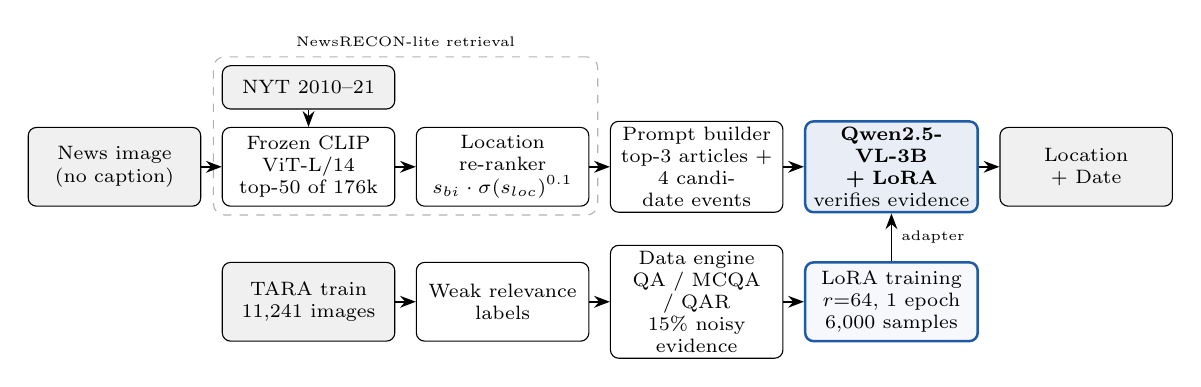
\begin{tikzpicture}[
  font=\scriptsize,
  box/.style={draw, rounded corners=3pt, align=center, minimum height=1.0cm, text width=2.05cm, inner sep=2pt},
  main/.style={box, draw=accent, fill=accent!10, line width=0.9pt},
  data/.style={box, fill=gray!12},
  arr/.style={-{Stealth[length=2mm]}, line width=0.6pt},
  node distance=0.35cm and 0.26cm]
\node[data] (img) {News image\\(no caption)};
\node[box, right=of img] (bi) {Frozen CLIP\\ViT-L/14\\top-50 of 176k};
\node[box, right=of bi] (ce) {Location\\re-ranker\\$s_{bi}\cdot\sigma(s_{loc})^{0.1}$};
\node[box, right=of ce] (pb) {Prompt builder\\top-3 articles +\\4 candidate events};
\node[main, right=of pb] (mllm) {\textbf{Qwen2.5-VL-3B}\\\textbf{+ LoRA}\\verifies evidence};
\node[data, right=of mllm] (out) {Location\\+ Date};
\node[data, below=0.7cm of bi] (tr) {TARA train\\11,241 images};
\node[box, right=of tr] (lab) {Weak relevance\\labels};
\node[box, right=of lab] (eng) {Data engine\\QA / MCQA / QAR\\15\% noisy evidence};
\node[main, right=of eng, fill=accent!4] (lora) {LoRA training\\$r{=}64$, 1 epoch\\6,000 samples};
\node[data, above=0.22cm of bi, minimum height=0.55cm] (corp) {NYT 2010--21};
\draw[arr] (img) -- (bi); \draw[arr] (bi) -- (ce); \draw[arr] (ce) -- (pb); \draw[arr] (pb) -- (mllm); \draw[arr] (mllm) -- (out);
\draw[arr] (corp) -- (bi);
\draw[arr] (tr) -- (lab); \draw[arr] (lab) -- (eng); \draw[arr] (eng) -- (lora); \draw[arr] (lora) -- node[right, font=\tiny]{adapter} (mllm);
\begin{scope}[on background layer]
\node[draw=gray!60, dashed, rounded corners, fit=(bi)(ce)(corp), inner sep=3pt, label={[font=\tiny]above:NewsRECON-lite retrieval}] {};
\end{scope}
\end{tikzpicture}

\vspace{0.6em}
\small
\begin{itemize}
\item \textbf{Retrieval:} frozen CLIP on headline + abstract; the location re-ranker's weight is tuned on dev
\item \textbf{Leakage control:} 2,734 TARA dev/test source articles removed from the corpus
\item \textbf{Model:} LoRA on all LM attention/MLP layers (3.1\% of the weights); vision encoder frozen
\end{itemize}
\end{frame}

% ---------------------------------------------------------------- 6
\begin{frame}{Proposed Methodology (2/2): Data Engine and Training Curve}
\begin{columns}[T]
\column{0.5\textwidth}
\small
\textbf{Three formats (LiveVQA), labels from retrieval}
\begin{itemize}
\item \textbf{QA:} image + top-3 articles $\rightarrow$ \texttt{Location / Date}
\item \textbf{MCQA:} options A--D = retrieved candidate events (hard negatives), E = ``none, use the image''
\item \textbf{QAR:} a verdict per article (same event / same place but other event / wrong place), then the answer
\end{itemize}
\textbf{Noisy evidence:} 15\% of samples get only irrelevant articles, so the model learns to \alert{reject} them\\[0.4em]
\textbf{Data:} 6,000 samples (1,769 QA, 2,406 MCQA, 1,825 QAR)\\
\textbf{Loss:} cross-entropy on answer tokens only
\column{0.47\textwidth}
\centering
\IfFileExists{figs/loss_curve.pdf}{%
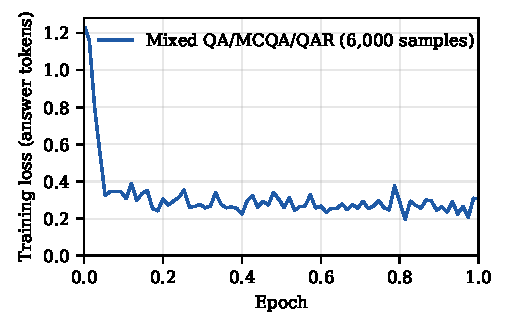
\includegraphics[width=\linewidth]{figs/loss_curve.pdf}}{%
\fbox{\parbox[c][4.2cm][c]{0.86\linewidth}{\centering\color{red}\small
PLACEHOLDER\\[0.3em] Training loss vs.\ epoch\\[0.3em]
\texttt{python scripts/plot\_loss.py}\\\texttt{\ \ \ \ loss\_log.json}\\[0.3em]
$\rightarrow$ upload \texttt{figs/loss\_curve.pdf}}}}
\\[0.2em]
{\scriptsize Training loss vs.\ epoch (1 epoch, 375 steps, effective batch 16): 1.23 $\rightarrow$ $\sim$0.33 in 20 steps, then plateaus}
\end{columns}
\end{frame}

% ---------------------------------------------------------------- 7
\begin{frame}{Experimental Setup}
\begin{columns}[T]
\column{0.5\textwidth}
\small
\textbf{Data}
\begin{itemize}
\item TARA: 12,306 train rows (11,241 images), 1,644 dev, 1,644 test
\item Test subset: 500 random images (471 with gold location, 432 with gold date)
\item Corpus: 176,314 NYT articles, 2010--2021
\end{itemize}
\textbf{Compared systems}
\begin{itemize}
\item Retrieval only: copy the top-1 article's metadata
\item Zero-shot Qwen2.5-VL-3B / 7B, with and without articles
\item Ours: LoRA, mixed formats; ablation: QA format only
\end{itemize}
\column{0.47\textwidth}
\small
\textbf{Training}
\begin{itemize}
\item Qwen2.5-VL-3B-Instruct, LoRA $r{=}64$, $\alpha{=}128$
\item AdamW, lr $10^{-4}$, cosine schedule, 1 epoch
\item Effective batch 16, bf16, images $\le 448^2$ pixels
\item $\sim$50 min on one 24\,GB GPU (peak 15\,GB)
\end{itemize}
\textbf{Metrics (NewsRECON)}
\begin{itemize}
\item \textbf{GREAT}: partial credit by date gap and km distance (0--100)
\item EM@1, Example-F1, $\Delta$, CO$\Delta$
\item Flips (blind-trust count), ECE (calibration)
\end{itemize}
\end{columns}
\end{frame}

% ---------------------------------------------------------------- 8
\begin{frame}{Results and Discussion (1/2): Main Results}
\begin{columns}[c]
\column{0.56\textwidth}
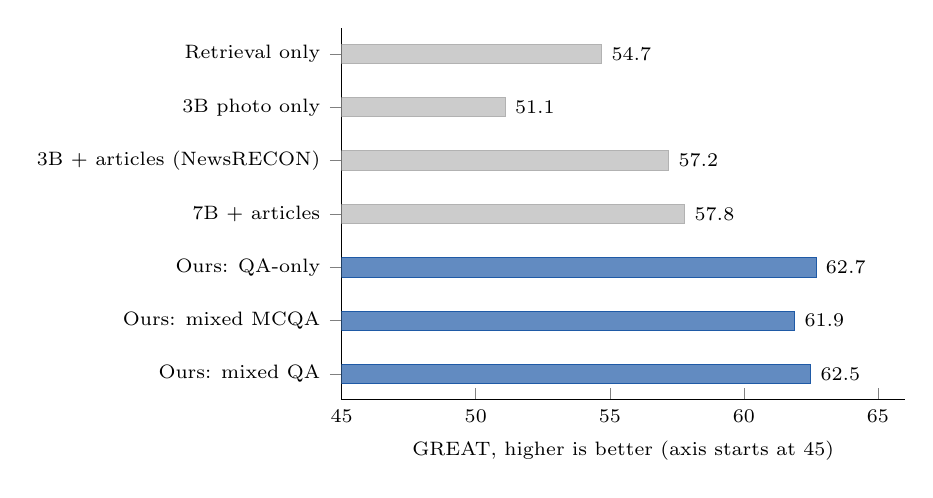
\begin{tikzpicture}
\begin{axis}[
  xbar, width=0.72\linewidth, height=6.3cm, bar shift=0pt,
  xmin=45, xmax=66, bar width=7pt,
  symbolic y coords={r,p,n,s,q,m,x},
  ytick={r,p,n,s,q,m,x}, yticklabels={Retrieval only,3B photo only,3B + articles (NewsRECON),7B + articles,Ours: QA-only,Ours: mixed MCQA,Ours: mixed QA}, y dir=reverse,
  yticklabel style={font=\scriptsize},
  xticklabel style={font=\scriptsize},
  xlabel={GREAT, higher is better (axis starts at 45)}, xlabel style={font=\scriptsize},
  nodes near coords, nodes near coords style={font=\scriptsize},
  enlarge y limits=0.08, axis x line*=bottom, axis y line*=left]
\addplot[fill=gray!40, draw=gray!60] coordinates {(54.7,r) (51.1,p) (57.2,n) (57.8,s)};
\addplot[fill=accent!70, draw=accent] coordinates {(62.7,q) (61.9,m) (62.5,x)};
\end{axis}
\end{tikzpicture}
\column{0.42\textwidth}
\small
\begin{itemize}
\item \textbf{+5.3 GREAT} over the NewsRECON setting (57.2 $\rightarrow$ 62.5)
\item Location EM@1: \textbf{31.4\% $\rightarrow$ 44.2\%}
\item Fine-tuned 3B \alert{beats zero-shot 7B} (57.8)
\item Zero-shot articles \alert{hurt} dates (GREAT$_{date}$ 59.0 $\rightarrow$ 57.6); after training, 64.9
\item Exact dates stay hard: EM@1 $\le$ 5.6\%
\end{itemize}
{\scriptsize Same 500 TARA test images and the same retrieved articles for all runs.}
\end{columns}
\end{frame}

% ---------------------------------------------------------------- 9
\begin{frame}{Results and Discussion (2/2): Blind Trust, Retrieval, Ablation}
\begin{columns}[T]
\column{0.48\textwidth}
\small
\textbf{Blind trust: location flips vs.\ photo-only 3B}\\
{\scriptsize C$\to$W = correct answer made wrong by articles}\\[0.3em]
\begin{tabular}{@{}lcc@{}}
\toprule
System & C$\to$W$\downarrow$ & W$\to$C$\uparrow$ \\
\midrule
Zero-shot 3B + articles & 29 & 61 \\
Zero-shot 7B + articles & 42 & 56 \\
\alert{Ours (mixed, QA)} & \alert{\textbf{7}} & \alert{\textbf{99}} \\
Ours (QA-only) & 4 & 96 \\
\bottomrule
\end{tabular}\\[0.6em]
\textbf{Retrieval (dev, location R@1)}\\[0.2em]
CLIP only 51.5 $\cdot$ re-ranker at $\alpha{=}1$: 51.0 $\cdot$ \textbf{$\alpha{=}0.1$: 55.1}
\column{0.48\textwidth}
\small
\textbf{Ablation and discussion}
\begin{itemize}
\item Blind-trust errors fall about \textbf{4$\times$} (29 $\rightarrow$ 7)
\item \textbf{QA-only $\approx$ mixed} (62.7 vs.\ 62.5) with 3.4$\times$ less data: the gain comes from training on \alert{noisy evidence}, not from the format mix
\item The MCQA output gives a usable confidence score: ECE 23.6 $\rightarrow$ 18.4
\item A light re-ranker helps; full weight (as in NewsRECON) hurts with frozen encoders
\end{itemize}
\end{columns}
\end{frame}

% ---------------------------------------------------------------- 10
\begin{frame}{Conclusion and Future Work}
\begin{columns}[T]
\column{0.5\textwidth}
\textbf{Conclusion}
\begin{itemize}
\small
\item NewsRECON-style retrieval + LiveVQA-style LoRA tuning on one GPU in about 1 hour
\item 3B model: \textbf{57.2 $\rightarrow$ 62.5 GREAT}, beating zero-shot 7B
\item Blind-trust errors reduced about 4$\times$
\item Training on noisy evidence matters more than model size or format mix
\end{itemize}
\column{0.47\textwidth}
\textbf{Future work}
\begin{itemize}
\small
\item Fine-tune the retriever on generated captions
\item Event-level re-ranking to improve exact dates
\item Evaluate on the full test set, 5Pils-OOC, and more seeds
\item Live news feed for images after 2021
\item News chatbot demo (built: Gradio app with evidence and follow-up questions)
\end{itemize}
\end{columns}
\end{frame}

% ---------------------------------------------------------------- 11
\begin{frame}{References}
\scriptsize
\begin{enumerate}
\item J. Tonglet, I. Gurevych, T. Tuytelaars, M.-F. Moens. NewsRECON: News article REtrieval for image CONtextualization. arXiv:2601.14121, 2026.
\item M. Fu, Y. Peng, D. Chen, Z. Zhou, B. Liu, et al. Seeking and updating with live visual knowledge. arXiv:2504.05288, 2025.
\item X. Fu, B. Zhou, I. Chandratreya, C. Vondrick, D. Roth. There's a time and place for reasoning beyond the image. ACL, 2022.
\item A. Radford et al. Learning transferable visual models from natural language supervision. ICML, 2021.
\item E. J. Hu et al. LoRA: Low-rank adaptation of large language models. ICLR, 2022.
\item S. Bai et al. Qwen2.5-VL technical report. arXiv:2502.13923, 2025.
\item S. Longpre et al. Entity-based knowledge conflicts in question answering. EMNLP, 2021.
\item J. Xie et al. Adaptive chameleon or stubborn sloth: Revealing the behavior of LLMs in knowledge conflicts. ICLR, 2024.
\item T. Zhang et al. RAFT: Adapting language model to domain specific RAG. COLM, 2024.
\item C. Guo, G. Pleiss, Y. Sun, K. Q. Weinberger. On calibration of modern neural networks. ICML, 2017.
\end{enumerate}
\end{frame}

\end{document}
